% This is samplepaper.tex, a sample chapter demonstrating the
% LLNCS macro package for Springer Computer Science proceedings;
% Version 2.20 of 2017/10/04
%
\documentclass[runningheads]{llncs}

\RequirePackage[
  % backend=bibtex,   % Recommended is `biber`, but gives
  backend=biber,     % timeout on Overleaf
  style=numeric,   % Equivalent to elsarticle-num-names
  sorting=none,    % Adjust sorting as needed
  natbib=true      % Compatibility with natbib
]{biblatex}

\usepackage{graphicx}
% \usepackage{cite}
\usepackage{url}
\usepackage{lipsum}                     % Dummytext
\usepackage{xargs}                      % Use more than one optional parameter in a new commands
\usepackage[pdftex,dvipsnames]{xcolor}  % Coloured text etc.
\usepackage{subcaption}


% Define custom colors
\definecolor{irrelevant}{RGB}{255, 0, 0} % Red color for old text
\definecolor{old}{RGB}{128, 128, 128} % Gray color for irrelevant text
\definecolor{final}{RGB}{0, 128, 0} % Green color for final text
\definecolor{edit}{RGB}{0, 0, 255} % Blue color for notes or other text


% Increase margin text width
\setlength{\marginparwidth}{2cm}

\usepackage{scrlayer-scrpage}

% Bibliography:
\addbibresource{bibliography/phd_proposal.bib}
\addbibresource{bibliography/lit_review_specific.bib}
\addbibresource{bibliography/zoom_calib.bib}

\setcounter{page}{1}


%
% ============== Define custom TODO commands ===========================
\usepackage[colorinlistoftodos,prependcaption,textsize=tiny, disable]{todonotes}

\newcommand{\comment}[2][Comment]{\todo[inline,color=blue!20!white]{\textbf{#1}: #2}}
\newcommand{\commentside}[2][Comment]{\todo[color=blue!20!white]{\textbf{#1}: #2}}
\newcommand{\fixme}[1]{%
  \todo[color=red!20, inline, size=\footnotesize]{FIXME: #1}%
}
\newcommand{\review}[1]{%
  \todo[color=blue!10, inline, size=\footnotesize]{REVIEW: #1}%
}

% With an exclamation mark icon
\newcommand{\alert}[1]{%
  \todo[inline, color=orange!30, size=\small, bordercolor=orange!80, linecolor=orange!80]{ALERT: #1}%
}

% ============== END: Define custom TODO commands ===========================

\makeatletter
\AtBeginDocument{%
  \def\doi#1{\url{https://doi.org/#1}}}
\makeatother

\makeatletter
\renewcommand\paragraph{\@startsection{paragraph}{4}{\z@}%
                                    {2.25ex \@plus1ex \@minus.2ex}%
                                    {-1em}%
                                    {\normalfont\normalsize\bfseries}}
\makeatother

%\urlstyle{same}

% Used for displaying a sample figure. If possible, figure files should
% be included in EPS format.
%
% If you use the hyperref package, please uncomment the following line
% to display URLs in blue roman font according to Springer's eBook style:
% \renewcommand\UrlFont{\color{blue}\rmfamily}

\begin{document}
%
\title{
  UGV Backtracking Recovery With Active Visual Landmarks Navigation:
  Literature Review (Assignment)
}

\author{Dmytro Kushnir\orcidID{0009-0006-8652-5781} }
%
\authorrunning{D. Kushnir}
% First names are abbreviated in the running head.
% If there are more than two authors, 'et al.' is used.
%
\institute{
  Ukrainian Catholic University, L'viv, Sventsitskogo st. 17,  79011, Ukraine
  \email{kushnir\_d@ucu.edu.ua}
}
%
\maketitle              % typeset the header of the contribution
%

\comment[does this type of work require "annotation" kind of block?]{}

% \keywords{
% Active localization \and
% Outdoor navigation \and
% Topological mapping \and
% Unstructured environment \and
% UGV \and
% Point of interest \and
% Visual landmarks \and
% GPS-denied operation
% }

% \end{abstract}

\section{Introduction}
Motivation for the topic of unstructured environments is multifaceted. Industries such as agriculture, mining, and military technology require advancements in autonomous systems, yet are hindered by the lack of open-source tools.
\todo{Elaborate on why open tools are pivotal for industry advancements and research progress.}

\textbf{Problem Statement:} Defining unstructured environments and their specific challenges will provide clarity. These environments lack predefined landmarks, pose navigation difficulties, and require robust adaptable systems.
\todo{Discuss what constitutes "unstructured environments" and why they are a significant research challenge.}

\section{Methodology}
This section outlines the approach to gathering and analyzing the literature.


\subsection{Specifc traits of domain literature}
\begin{itemize}
  \item Inclusion of large-scale reviews or almanacs (250+ papers for aggregation).
  \item Amount of publications are orders of magnitude lower than in mainstream AI.
  \item Challenge-based (DARPA, MBZIRC) research initiatives. "Clusters" of connected around single problem.
  \item Long-term researches done by large, well established teams.
  \item Lack of benchmarks or datasets.
\end{itemize}

From this we derive conclusion that snowballing approach is not the most effective in those field. Instead regular almanacs, big reviews, and challenge-based researches are sufficient to give navigation in the field.

\begin{figure}[ht]
  \centering
  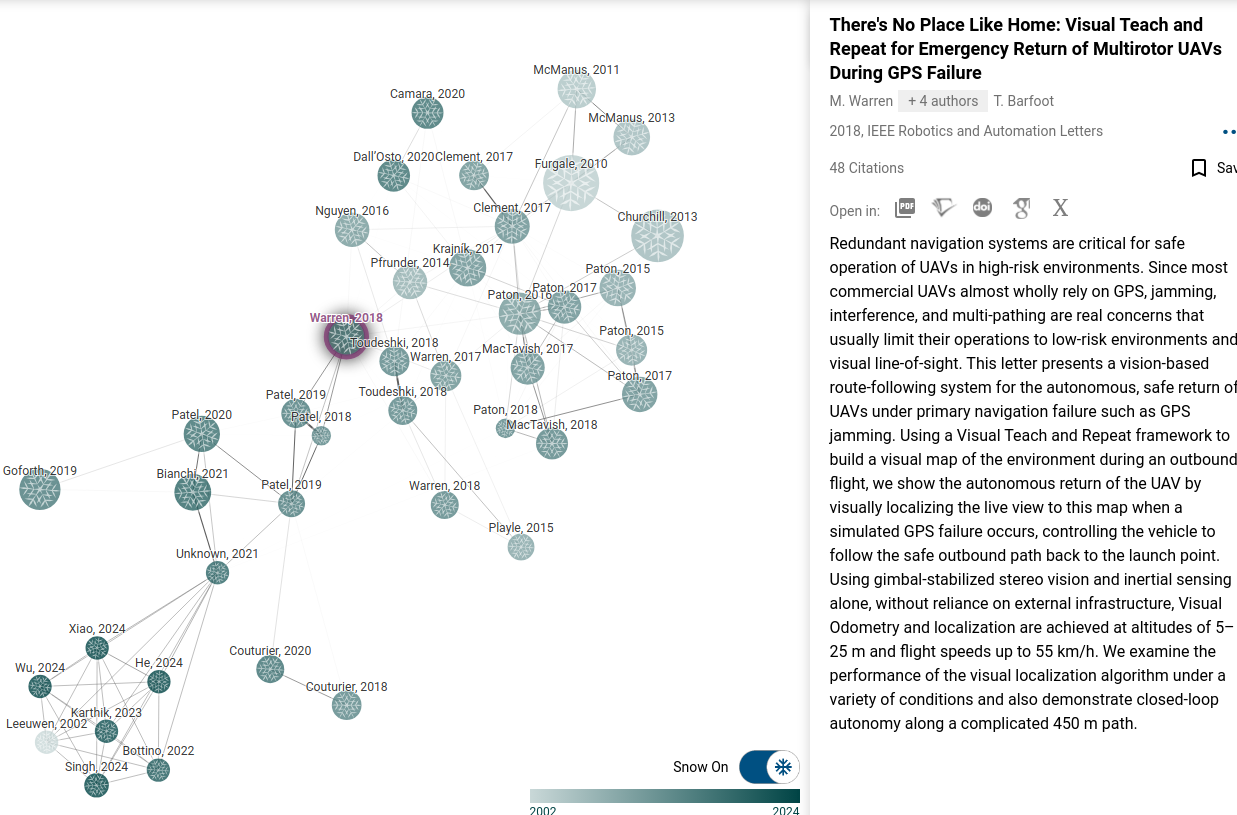
\includegraphics[width=\linewidth]{img/There_is_no_place_like_home_research_tree.png}
  \caption{Visual Teach-and-Repeat approach for emergency return of multirotor UAVs during GPS failure \cite{warren-ral19-no-place-like-Home}. More information is available on Connected Papers: \protect\url{https://www.connectedpapers.com/}.}
  \label{fig:no_place_like_home}
\end{figure}

Naturally, as problems in a field of robotics include lots of disection reasons: indoor/outdoor, aerial/ground, realtime/non-realtime, etc. -- answering all those quelification questions mean that the tackable "frontier" of research is pin-tip scale. It is marely enough community members to place the large-scale benchmarks and meaningful datasets. This is one of the reasons , why the problems are usually condensed to obvious tasks, that happen to lie beyond the frontiers of modern robotics. "Returning back home" is one of such an everyday problems.
Sinse there is not much place for terminological mislabeling of such a tasks,  it is easy to find the track of the relevant papers. They are always clustered around research centers, datasets or individual experts. Subsequently, we marely can expect to see the terminological saturation in the field of particular, defined problem. The most cited papers in field of Robotics rarely have 500+ citations ("FastSLAM: A factored solution to the simultaneous localization and mapping problem" (2002): ~3,500 citations in 20 years.) , while for AI the 50'000 citations are not incredible anymore ("BERT: Pre-training of Deep Bidirectional Transformers for Language Understanding" (2018): ~50,000 citations by 2023.). Therefore the scale of the task is not large enough for the snowballing approach.

 The papers are well connected, and the research is done in the "clusters" of research groups. The example of such is the work of Warren et al. \ref{fig:no_place_like_home} and we see here the modest in size and tight in connections are the works in the field.
Classic citation network analysis is not the best tool for the field, as the papers are well connected and the clusters are small.

Thing that metters here is the formulation of the problem, the requirements, that are solved by the design of the solution. The implementation and validation are the next steps, that replace the "benchmarks" in the field of robotics.

\comment[Here we will meticulously deconstruct the whole challange into set of requirements, investigate the available set of apporaches, tradeoffs and design the solution aspects. The CORE of literature analysis in robotics will be here. In such a manner we will ensure that we are solving the actual large-scale problem applicable beyond our setup. ]{}

\subsection{Selection Criteria}
\begin{itemize}
  \item Availability of implementations adaptable for our platform or published ground truth data.
  \item Papers demonstrating superior benchmark performance.
        \todo{Incorporate specific sources or frameworks, e.g., S. Hausler et al., 2024.}
  \item Industry standards and tools with robust GitHub presence.
\end{itemize}


\subsection{Analysis Framework}
The review leverages a structured "Task-Requirement-Design-Implementation-Validation" methodology.
\todo{Include visual diagrams or reference placeholders for MeROS-based design layers.}

Challenges-based research in robotics emphasizes organized progress, such as DARPA competitions, driving iterative advancements in solutions.
\todo{Amplify with examples of explosive technology disruptions, e.g., Kinect or ROS2.}

\section{State-of-the-Art}

\comment{Larger piece for ROS. Other will be detailed in similar fashion + references}

\subsection{The Critical Role of the ROS Platform}
The Robot Operating System (ROS) has emerged as a cornerstone technology in the robotics field, providing an open-source framework that standardizes development and fosters collaboration across academia and industry. Its modular architecture allows researchers and developers to integrate diverse hardware and software components, enabling rapid prototyping and scalability for a wide range of applications.

One of ROS's most significant contributions is its community-driven ecosystem, where shared libraries, tools, and documentation accelerate innovation. ROS supports real-time applications, bridging the gap between laboratory research and field deployment. This feature has proven particularly valuable in unstructured environments, where dynamic conditions demand robust and flexible solutions. Moreover, the adoption of ROS by industry leaders has enhanced its relevance, making it a platform that seamlessly connects academic research with practical deployment.

In the context of this review, ROS plays a pivotal role in the development of modular designs, such as the MeROS framework. By leveraging ROS's tools for sensor integration, motion planning, and communication, MeROS exemplifies how a standardized platform can streamline the design and validation of complex robotic systems. However, despite its strengths, ROS is not without limitations. Challenges such as real-time processing constraints, hardware compatibility, and dependency management persist, leaving room for further enhancements.

\subsection{Mapping Approaches}
Summarize current techniques in mapping for unstructured environments.
\todo{Discuss strengths and limitations of existing methods.}

\subsection{Visual Perception and PTZ Cameras}
Discuss the role of PTZ cameras in UGV platforms, emphasizing modular design and requirement-based development.
\todo{Include examples of modular designs and calibrations.}

\subsection{Public and Private SOTA}
Contrast public SOTA with proprietary solutions. Highlight the reproducibility crisis in robotics academia due to platform-locked tools.
\todo{Explore the coined term "Public SOTA" and its implications.}

\section{Research Gaps}
\subsection{Task-Requirement-Design Identification}

Core research gaps
\comment[We will concentrate our research efforts on them specifically]{}

\begin{itemize}
  \item PTZ camera integration challenges.
  \item Long-range navigation in unstructured environments:
        \begin{itemize}
          \item Representation of places.
          \item Route following between places with minimal memorization.
        \end{itemize}
  \item Encapsulation of independent software-hardware modules.
  \item Cross-platform interfacing and requirements management.
  \item Calibration and processing for open-source tools.
\end{itemize}
\todo{Explore solutions like 360-degree cameras or alternative configurations.}

\subsection{Constraints and Challenges}
\comment[Those are factors that can have decisive impact on feasibility of the work and they require our attention, but those fell out of the main focus of the research]{}

\begin{itemize}
  \item Planning and power management.
        Long-range navigation is limited by the energy capacity of the UGV and the efficiency of its spending.
  \item Environmental factors such as weather, light, and terrain complexity.
        This parameter has to be mentioned, to clearly denote limitations of considered conditions.
  \item Real-time processing requirements.
        The real-time processing of sensor data and decision-making are important for the robotisc, but we outline the problem and design solution in such a manner to allow for the relaxations on this requirement.
  \item Scalability and integration with ROS platforms.
        As we touch lots of system aspects with limited resources, we will focus on the iterative implementations and open solutions.
\end{itemize}
\todo{Discuss relaxations on real-time requirements and focus on iterative implementations.}

\section{Conclusion and Motivation}
The proposed research aims to:
\begin{itemize}
  \item Emphasize modular design and cross-platform usability.
  \item Identify critical bottlenecks halting advancements.
  \item Validate the feasibility of addressing these bottlenecks through:
        \begin{itemize}
          \item Open-source calibration and integration tools.
          \item Testing on Husky UGV or equivalent platforms.
          \item Clear documentation and interfaces following MeROS philosophy.
        \end{itemize}
\end{itemize}
\todo{Highlight the significance of open-source contributions and iterative validation in advancing the field.}

\section{Datasets and Resources}
A few datasets can serve as a basis for this research or as a sign of missing data:
\begin{itemize}
  \item Wild Scenes Dataset: \url{https://arxiv.org/pdf/2404.18477}
  \item Wild Places Dataset: \url{https://csiro-robotics.github.io/Wild-Places}
  \item Freiburg Forest: \url{https://paperswithcode.com/dataset/freiburg-forest}
\end{itemize}
\todo{Note the gaps in available datasets and propose directions for addressing these limitations.}


\printbibliography


\end{document}
```
